\documentclass[10pt,letterpaper,unboxed,cm]{exam}
\usepackage[margin=1in]{geometry}
\usepackage{amsmath,mathabx}
\usepackage{color}
\usepackage{mdframed}
\usepackage{graphicx}
\usepackage{changepage}
\usepackage[skip=8pt]{parskip}
\usepackage{booktabs}
\usepackage{enumitem}



\begin{document}



% HEADER
\setlength{\parskip}{4pt}
\hfill{OpenIntro Statistics - 4th Edition}

\hfill{Chapter 2 Exercises}

\hfill{December 26, 2024}

\hfill{ODD SOLUTIONS}
\setlength{\parskip}{8pt}
\rule{\linewidth}{2pt}
% HEADER



\begin{questions}



% QUESTION 1
	\question \underline{2.1 Mammal life spans.}

    Data were collected on life spans (in years) and gestation lengths (in days) for 62 mammals. A scatterplot of life span versus length of gestation is shown below.

    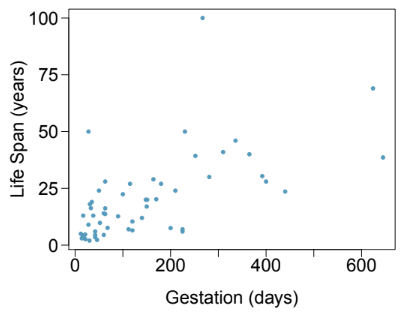
\includegraphics[width=0.5\textwidth]{exercise21.png}
    
	\begin{parts}
		\part What type of an association is apparent between life span and length of gestation?
        
        \bigskip
        {\bf There is a positive, linear association.} 
        \bigskip

		\part What type of an association would you expect to see if the axes of the plot were reversed, i.e. if we plotted length of gestation versus life span?
        
        \bigskip
        {\bf We would see the same type of association except the linear line would be more steeper.} 
        \bigskip

		\part Are life span and length of gestation independent? Explain your reasoning.
        
        \bigskip
        {\bf No, the scatterplot suggests a relationship between these two variables in the fact that increasing one variable leads to an increase in the second one as well.} 
        \bigskip
	\end{parts}
% QUESTION 1



% QUESTION 2
	\question \underline{2.3 Reproducing bacteria.}

    Suppose that there is only sufficient space and nutrients to support one million bacterial cells in a petri dish. You place a few bacterial cells in this petri dish, allow them to reproduce freely, and record the number of bacterial cells in the dish over time. Sketch a plot representing the relationship between number of bacterial cells and time.

    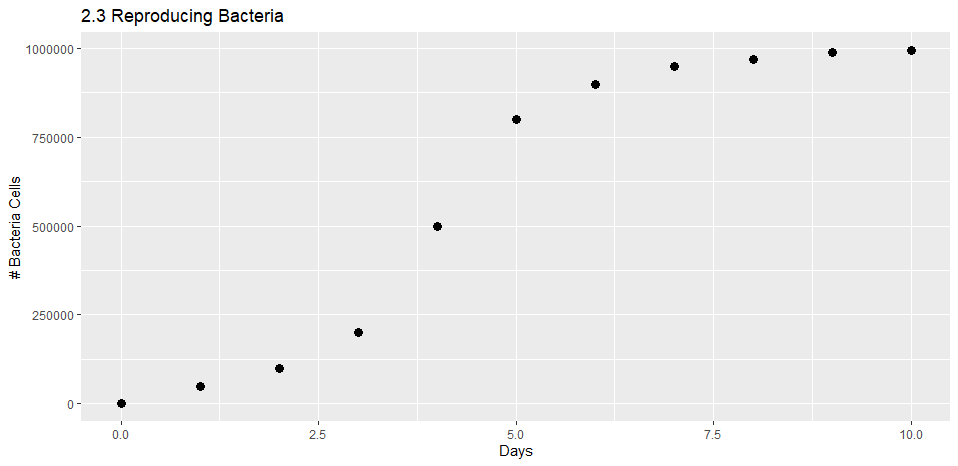
\includegraphics[width=\textwidth]{23scatterplot.png}
% QUESTION 2



% QUESTION 3
	\question \underline{2.5 Parameters and statistics.}

    Identify which value represents the sample mean and which value represents the claimed population mean.
    
	\begin{parts}
		\part American households spent an average of about \$52 in 2007 on Halloween merchandise such as costumes, decorations and candy. To see if this number had changed, researchers conducted a new survey in 2008 before industry numbers were reported. The survey included 1,500 households and found that average Halloween spending was \$58 per household.
        
        \bigskip
        {\bf
            \begin{itemize}
                \item Sample mean: \$58
                \item Population mean: \$52
            \end{itemize}
        } 
        \bigskip

		\part The average GPA of students in 2001 at a private university was 3.37. A survey on a sample of 203 students from this university yielded an average GPA of 3.59 a decade later.
        
        \bigskip
        {\bf
            \begin{itemize}
                \item Sample mean: 3.59
                \item Population mean: 3.37
            \end{itemize}
        } 
        \bigskip
	\end{parts}
% QUESTION 3



% QUESTION 4
	\question \underline{2.7 Days off at a mining plant.}

    Workers at a particular mining site receive an average of 35 days paid vacation, which is lower than the national average. The manager of this plant is under pressure from a local union to increase the amount of paid time off. However, he does not want to give more days off to the workers because that would be costly. Instead he decides he should fire 10 employees in such a way as to raise the average number of days off that are reported by his employees. In order to achieve this goal, should he fire employees who have the most number of days off, least number of days off, or those who have about the average number of days off?
    
    \bigskip
    {\bf He should fire employees who have the least number of days off. The goal is to increase the mean value of number of days off so removing values below the current mean would increase the value of the mean.} 
    \bigskip
% QUESTION 4



% QUESTION 5
	\question \underline{2.9 Means and SDs.}

    For each part, compare distributions (1) and (2) based on their means and standard deviations. You do not need to calculate these statistics; simply state how the means and the standard deviations compare. Make sure to explain your reasoning. Hint: It may be useful to sketch dot plots of the distributions.
    
	\begin{parts}
		\part (1) 3, 5, 5, 5, 8, 11, 11, 11, 13\\(2) 3, 5, 5, 5, 8, 11, 11, 11, 20
        
        \bigskip
        {\bf Both the mean and standard deviation of (2) are greater than (1).} 
        \bigskip

		\part (1) -20, 0, 0, 0, 15, 25, 30, 30\\(2) -40, 0, 0, 0, 15, 25, 30, 30
        
        \bigskip
        {\bf Both the mean and standard deviation of (1) are greater than (2).} 
        \bigskip

		\part (1) 0, 2, 4, 6, 8, 10\\(2) 20, 22, 24, 26, 28, 30
        
        \bigskip
        {\bf The standard deviation is the same for (1) and (2). The mean for (1) is less than (2).} 
        \bigskip

		\part (1) 100, 200, 300, 400, 500\\(2) 0, 50, 300, 550, 600
        
        \bigskip
        {\bf (1) and (2) share the same mean. (2) has the greater standard deviation.} 
        \bigskip

	\end{parts}
% QUESTION 5



% QUESTION 6
	\question \underline{2.11 Air quality.}

    Daily air quality is measured by the air quality index (AQI) reported by the Environ- mental Protection Agency. This index reports the pollution level and what associated health effects might be a concern. The index is calculated for five major air pollutants regulated by the Clean Air Act and takes values from 0 to 300, where a higher value indicates lower air quality. AQI was reported for a sample of 91 days in 2011 in Durham, NC. The relative frequency histogram below shows the distribution of the AQI values on these days.

    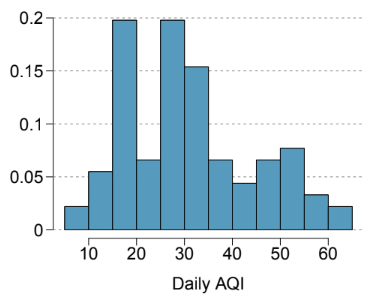
\includegraphics[width=0.5\textwidth]{exercise211.png}
    
	\begin{parts}
		\part Estimate the median AQI value of this sample.
        
        \bigskip
        {\bf Between 25 and 35.} 
        \bigskip

		\part Would you expect the mean AQI value of this sample to be higher or lower than the median? Explain your reasoning.
        
        \bigskip
        {\bf I would expect the mean value of this sample to be lower than the median. There are two distinct peaks in this sample located in the lower half of the sample, making it a bimodal plot. Since the peaks are in the lower half of the graph, there are more smaller values making the mean lower than the median.} 
        \bigskip

		\part Estimate Q1, Q3, and IQR for the distribution.
        
        \bigskip
        {\bf Q1: 20, Q3: 40, IQR: 20} 
        \bigskip

		\part Would any of the days in this sample be considered to have an unusually low or high AQI? Explain your reasoning.
        
        \bigskip
        {\bf No. The lowest and highest values of this distribution have neighboring values with similar frequencies.} 
        \bigskip

	\end{parts}
% QUESTION 6



% QUESTION 7
	\question \underline{2.13 Histograms vs. box plots.}

    Compare the two plots below. What characteristics of the distribution are apparent in the histogram and not in the box plot? What characteristics are apparent in the box plot but not in the histogram?

    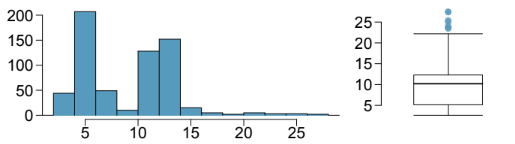
\includegraphics[width=\textwidth]{exercise213.png}

    \bigskip
    {\bf In the histogram the two peaks and mode value are apparent but the outliers are not. In the box plot the outliers are made apparent through the points outside of the IQR and whiskers and the median is apparent as well where in the histogram it is not.} 
    \bigskip
% QUESTION 7



% QUESTION 8
	\question \underline{2.15 Distributions and appropriate statistics, Part I.}

    For each of the following, state whether you expect the distribution to be symmetric, right skewed, or left skewed. Also specify whether the mean or median would best represent a typical observation in the data, and whether the variability of observations would be best represented using the standard deviation or IQR. Explain your reasoning.
    
	\begin{parts}
		\part Number of pets per household.
        
        \bigskip
        {\bf
            \begin{itemize}
                \item Distribution: Right skewed because it is more uncommon to have a higher number of pets.
                \item Typical observation: Median since the data is skewed and the median is more stable than the mean value.
                \item Variability: IQR for similar reasons as the typical observation. The IQR is influenced less by outliers and skewed distributions
            \end{itemize}
        } 
        \bigskip

		\part Distance to work, i.e. number of miles between work and home.
        
        \bigskip
        {\bf
            \begin{itemize}
                \item Distribution: Right skewed because people tend to live closer to their place of work and less commonly the farther away from work.
                \item Typical observation:  Median since the data is skewed and the median value is more resilient to outliers and skewness.
                \item Variability: IQR for the same reasons above.
            \end{itemize}
        } 
        \bigskip

		\part Heights of adult males.
        
        \bigskip
        {\bf
            \begin{itemize}
                \item Distribution: Symmetrical because the heights of males is well centered around an average height. 
                \item Typical observation: Mean because the distribution is symmetrical.
                \item Variability: Standard deviation since the data is symmetrical.
            \end{itemize}
        } 
        \bigskip
	\end{parts}
% QUESTION 8



% QUESTION 9
	\question \underline{2.17 Income at the coffee shop.}

    The first histogram below shows the distribution of the yearly incomes of 40 patrons at a college coffee shop. Suppose two new people walk into the coffee shop: one making \$225,000 and the other \$250,000. The second histogram shows the new income distribution. Summary statistics are also provided.

    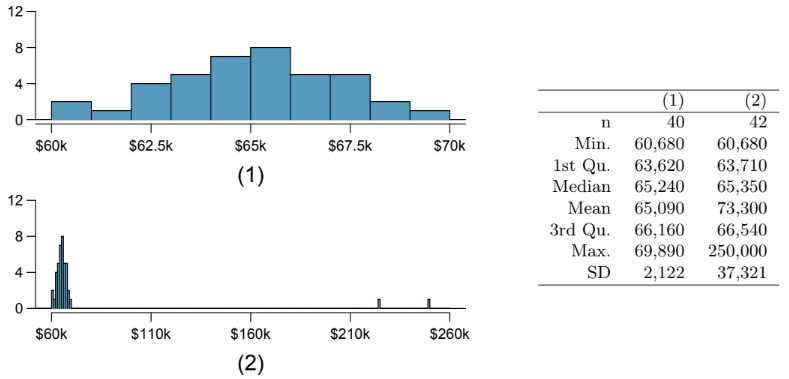
\includegraphics[width=\textwidth]{exercise217.png}
    
	\begin{parts}
		\part Would the mean or the median best represent what we might think of as a typical income for the 42 patrons at this coffee shop? What does this say about the robustness of the two measures?
        
        \bigskip
        {\bf The median would best represent the typical income since the last two patrons act as extreme outliers. This shows that the median value is most robust to outliers compared to the mean value.} 
        \bigskip

		\part Would the standard deviation or the IQR best represent the amount of variability in the incomes of the 42 patrons at this coffee shop? What does this say about the robustness of the two measures?
        
        \bigskip
        {\bf The IQR is clearly a better representation of the variability in the incomes since the last two outliers increases the standard deviation by about $3,5000$.}wa
        \bigskip
	\end{parts}
% QUESTION 9



% QUESTION 10
	\question \underline{2.19 Commute times.}

    The US census collects data on time it takes Americans to commute to work, among many other variables. The histogram below shows the distribution of average commute times in 3,142 US counties in 2010. Also shown below is a spatial intensity map of the same data.

    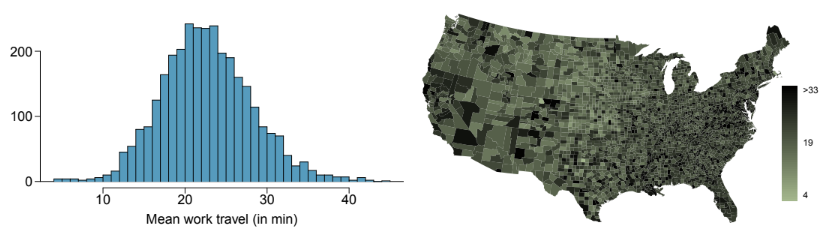
\includegraphics[width=\textwidth]{exercise219.png}
    
	\begin{parts}
		\part Describe the numerical distribution and comment on whether or not a log transformation may be advisable for these data.
        
        \bigskip
        {\bf The distribution is already symmetrical and well centered so the log transformation is not needed to transform the skewness. If you care about bringing the lower and higher values of the distribution closer to the center, the log transformation could help with reducing the spread/variation.} 
        \bigskip

		\part Describe the spatial distribution of commuting times using the map above.
        
        \bigskip
        {\bf The map shows a spatial distribution with smaller values towards the middle of the country and higher values towards the borders.} 
        \bigskip
	\end{parts}
% QUESTION 10



% QUESTION 11
	\question \underline{2.21 Antibiotic use in children.}

    The bar plot and the pie chart below show the distribution of pre-existing medical conditions of children involved in a study on the optimal duration of antibiotic use in treatment of tracheitis, which is an upper respiratory infection.

    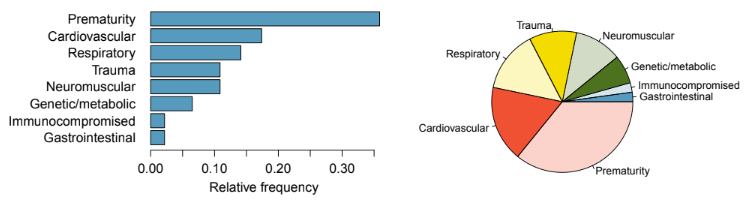
\includegraphics[width=\textwidth]{exercise221.png}
    
	\begin{parts}
		\part What features are apparent in the bar plot but not in the pie chart?
        
        \bigskip
        {\bf Features such as the mode (Prematurity) of the distribution and the relative differences between the frequencies of medical condition is apparent in the bar plot but not in the pie chart.} 
        \bigskip

		\part What features are apparent in the pie chart but not in the bar plot?
        
        \bigskip
        {\bf The pie chart makes it apparent that the distributions are all standardized as ratios of a whole.} 
        \bigskip

		\part Which graph would you prefer to use for displaying these categorical data?
        
        \bigskip
        {\bf I would prefer the bar plot because the pie chart does not offer any advantages that the the bar plot does not, such as relative frequencies, while being more confusing.} 
        \bigskip
	\end{parts}
% QUESTION 11



% QUESTION 12
	\question \underline{2.23 Views on the DREAM Act.}

    A random sample of registered voters from Tampa, FL were asked if they support the DREAM Act, a proposed law which would provide a path to citizenship for people brought illegally to the US as children. The survey also collected information on the political ideology of the respondents. Based on the mosaic plot shown below, do views on the DREAM Act and political ideology appear to be independent? Explain your reasoning.

    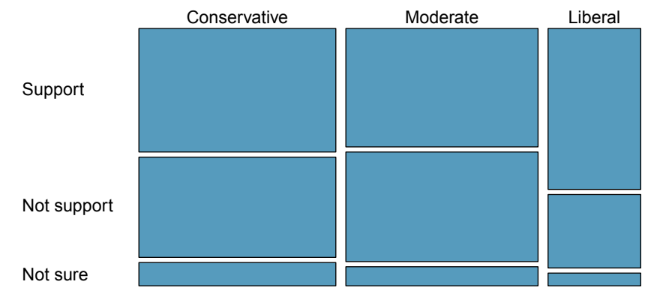
\includegraphics[width=\textwidth]{exercise223.png}
    
    \bigskip
    {\bf No, the mosaic plot seems to suggest that the political ideologies and stances on the DREAM act of respondents are associated. The ratios of stances across the three political ideologies vary slightly which means that the two variables are most likely not independent.} 
    \bigskip
% QUESTION 12



% QUESTION 13
	\question \underline{2.25 Side effects of Avandia.}

    Rosiglitazone is the active ingredient in the controversial type 2 diabetes medicine Avandia and has been linked to an increased risk of serious cardiovascular problems such as stroke, heart failure, and death. A common alternative treatment is pioglitazone, the active ingredient in a diabetes medicine called Actos. In a nationwide retrospective observational study of 227,571 Medicare beneficiaries aged 65 years or older, it was found that 2,593 of the 67,593 patients using rosiglitazone and 5,386 of the 159,978 using pioglitazone had serious cardiovascular problems. These data are summarized in the contingency table below.

    \begin{table}[ht]
    \centering
    \begin{tabular}{lccc}
       & \multicolumn{2}{c}{\textit{Cardiovascular problems}} & \\
       \cmidrule(lr){2-3}
       & Yes & No & Total\\
       \midrule
       \makebox[0pt][r]{\textit{Treatment}\quad}Rosiglitazone & 2,593 & 65,000 & 67,593 \\
       Pioglitazone                                         & 5,386 & 154,592 & 159,978 \\
       \midrule
       Total                                           & 7,979 & 219,592 & 227,571 \\
    \end{tabular}
    \end{table}
    
	\begin{parts}
		\part Determine if each of the following statements is true or false. If false, explain why. Be careful: The reasoning may be wrong even if the statement’s conclusion is correct. In such cases, the statement should be considered false.

        \begin{enumerate}[label=\roman*.]
            \item Since more patients on pioglitazone had cardiovascular problems (5,386 vs. 2,593), we can conclude that the rate of cardiovascular problems for those on a pioglitazone treatment is higher.
                    
            \bigskip
            {\bf This statement is false because the values $5,386$ and $2,593$ cannot be directly compared since the sample size of each group has a large difference. Instead, the ratio of patients who suffered and didn't suffer from cardiovascular problems for each group should be compared.} 
            \bigskip

            \item The data suggest that diabetic patients who are taking rosiglitazone are more likely to have cardiovascular problems since the rate of incidence was $(2,593 / 67,593 = 0.038)~3.8\%$ for patients on this treatment, while it was only (5,386 / 159,978 = 0.034) 3.4\% for patients on pioglitazone.
        
            \bigskip
            {\bf This statement is false. While the ratio is technically smaller for patients taking pioglitazone, the difference is only 0.4\%. This small difference may be due to random chance.} 
            \bigskip

            \item The fact that the rate of incidence is higher for the rosiglitazone group proves that rosiglitazone causes serious cardiovascular problems.
        
            \bigskip
            {\bf This statement is false. While it may be true that rosiglitazone could cause serious cardiovascular problems, a comparison of these two ratios does not prove it.} 
            \bigskip

            \item Based on the information provided so far, we cannot tell if the difference between the rates of incidences is due to a relationship between the two variables or due to chance.
        
            \bigskip
            {\bf True.} 
            \bigskip
        \end{enumerate}

		\part What proportion of all patients had cardiovascular problems?
        
        \bigskip
        {\bf $7,979 / 227,571 \approx 0.035 = 3.5\%$} 
        \bigskip

		\part If the type of treatment and having cardiovascular problems were independent, about how many patients in the rosiglitazone group would we expect to have had cardiovascular problems?
        
        \bigskip
        {\bf We would expect about 3.5\% of any group of people in this sample to have cardiovascular problems assuming the variables were independent.
        
         3.5\% of 67,593 amounts to $67,593 \times 0.035 \approx 2366$ people which is very close to the actual amount observed in the experiment.}
        \bigskip

		\part We can investigate the relationship between outcome and treatment in this study using a randomization technique. While in reality we would carry out the simulations required for randomization using statistical software, suppose we actually simulate using index cards. In order to simulate from the independence model, which states that the outcomes were independent of the treatment, we write whether or not each patient had a cardiovascular problem on cards, shuffled all the cards together, then deal them into two groups of size 67,593 and 159,978. We repeat this simulation 1,000 times and each time record the number of people in the rosiglitazone group who had cardiovascular problems. Use the relative frequency histogram of these counts to answer (i)-(iii).

        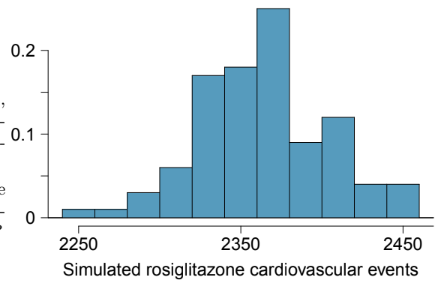
\includegraphics[width=0.5\textwidth]{exercise225.png}
        
        \begin{enumerate}[label=\roman*.]
            \item What are the claims being tested?
                    
            \bigskip
            {\bf
                \begin{itemize}
                    \item Independence Model: The treatments have no affect on cardiovascular problems, and we just happened to observe a small difference that would occur by chance.
                    \item Alternative Model: The treatments have an effect on cardiovascular problems, and the small difference we observe was actually due to rosiglitazone causing more cardiovascular problems.
                \end{itemize}
            } 
            \bigskip

            \item Compared to the number calculated in part (c), which would provide more support for the alternative hypothesis, {\it more} or {\it fewer} patients with cardiovascular problems in the rosiglitazone group?
        
            \bigskip
            {\bf We would need more patients with cardiovascular problems in the rosiglitazone group since the current ratio is in the center of the simulated distribution which supports the independence model.} 
            \bigskip

            \item What do the simulation results suggest about the relationship between taking rosiglitazone and having cardiovascular problems in diabetic patients?
        
            \bigskip
            {\bf The simulated results suggest that the two variables have an independent relationship since the observed ratio of 3.8\% fits in a commonly observed bin of values in the simulation.} 
            \bigskip
        \end{enumerate}

	\end{parts}
% QUESTION 13



\end{questions}
\end{document}